\documentclass[a4paper,12pt]{article}
\usepackage{amsmath,amsfonts,siunitx}
\usepackage{geometry}
\usepackage{graphicx}
\usepackage{booktabs}
\usepackage{hyperref}
\usepackage{enumitem}

% Comandos personalizados para citações
\newcommand{\citeonline}[1]{\textbf{#1}}
\usepackage[utf8]{inputenc}
\usepackage[T1]{fontenc}
\usepackage{indentfirst}
\usepackage{tikz}
\usetikzlibrary{calc, positioning, arrows.meta}
\geometry{margin=2.5cm}
\sisetup{locale = FR, per-mode=symbol, separate-uncertainty = true}

\title{Análise Reológica de Pastas Cerâmicas}
\author{Bruno Kenji Nishitani Egami}
\date{}
\usepackage{helvet}
\renewcommand{\familydefault}{\sfdefault}

\begin{document}
\maketitle
\href{https://github.com/bruno-egami/Reometro_Capilar/tree/Reometro-capilar-Transdutor_Pasta}{\textbf{Link para o projeto}}

\section*{1. Introdução}
A caracterização reológica de pastas cerâmicas é essencial para entender seu comportamento durante processos de conformação, como a extrusão. O presente relatório descreve as equações utilizadas em um script Python desenvolvido para processar os dados experimentais obtidos com um reômetro capilar DIY de baixo custo. O objetivo é converter medidas diretas (como massa extrudada e pressão de extrusão) em parâmetros reológicos interpretáveis (como viscosidade e taxa de cisalhamento).

\subsection*{1.1 Aplicações em Manufatura Aditiva}
O controle reológico preciso é fundamental para tecnologias emergentes como a impressão 3D cerâmica, especialmente na técnica \textit{Direct Ink Writing} (DIW) ou \textit{Robocasting}. Esta técnica requer pastas com comportamento pseudoplástico que fluam sob cisalhamento (extrusão pelo bico), mas recuperem rapidamente sua viscosidade após a deposição para suportar as camadas subsequentes (\textit{buildability}). A caracterização sistemática do comportamento reológico da matéria-prima base é, portanto, um pré-requisito para o desenvolvimento de formulações otimizadas para manufatura aditiva.

\subsection*{1.2 Histórico de Desenvolvimento do Equipamento}
O reômetro capilar utilizado neste estudo é resultado de um processo evolutivo de três gerações:

\begin{itemize}
  \item \textbf{V1 (Protótipo Inicial):} A primeira versão utilizava medição indireta de pressão através de uma célula de carga (extensômetros e módulo HX711). Esta configuração permitia estimar a força aplicada durante a extrusão. O sistema foi validado experimentalmente demonstrando boa concordância com reômetros comerciais.
  
  \item \textbf{V2 (Transdutor Único):} Na segunda geração, a célula de carga foi substituída por um transdutor de pressão de linha (faixa de 0-150 psi) para leitura direta da pressão do ar comprimido. Esta modificação simplificou o sistema e melhorou a precisão das medições.
  
  \item \textbf{V3 (Atual - Duplo Transdutor):} A versão atual incorpora um segundo transdutor posicionado diretamente na câmara da pasta (sensor "Pasta"), além do transdutor de linha (sensor "Linha"). Esta configuração permite eliminar erros sistemáticos causados pelo atrito do pistão e possibilita a aplicação mais precisa das correções de Bagley e Mooney, fundamentais para fluidos não-Newtonianos.
\end{itemize}

\begin{figure}[htbp]
\centering
\resizebox{0.95\textwidth}{!}{%
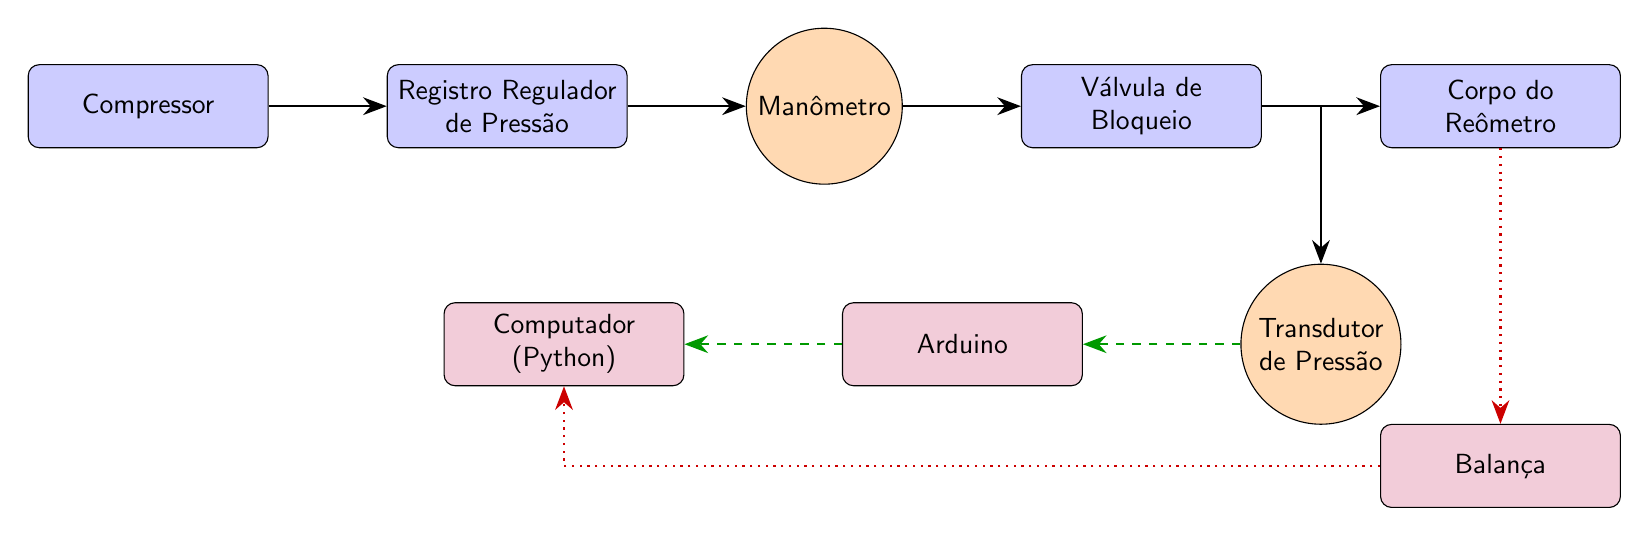
\begin{tikzpicture}[node distance=2cm, auto]
    \usetikzlibrary{calc, positioning}
    
    \tikzstyle{block} = [rectangle, draw, fill=blue!20, text width=8em, text centered, rounded corners, minimum height=3em]
    \tikzstyle{instrument} = [circle, draw, fill=orange!30, text centered, minimum size=5em, align=center]
    \tikzstyle{data_block} = [rectangle, draw, fill=purple!20, text width=8em, text centered, rounded corners, minimum height=3em]
    \tikzstyle{line} = [draw, thick, -{Stealth[length=3mm]}]
    \tikzstyle{data_line} = [draw, thick, dashed, color=green!60!black, -{Stealth[length=3mm]}]
    \tikzstyle{manual_line} = [draw, thick, dotted, color=red!80!black, -{Stealth[length=3mm]}]
    
    \node [block] (compressor) {Compressor};
    \node [block, right=1.5cm of compressor] (regulator) {Registro Regulador de Pressão};
    \node [instrument, right=1.5cm of regulator] (manometer) {Manômetro};
    \node [block, right=1.5cm of manometer] (valve) {Válvula de Bloqueio};
    \node [block, right=1.5cm of valve] (rheometer) {Corpo do Reômetro};
    
    \coordinate (tap_point) at ($(valve.east)!0.5!(rheometer.west)$);
    
    \node [instrument, below=2cm of tap_point] (transducer) {Transdutor \\ de Pressão};
    \node [data_block, left=2cm of transducer] (arduino) {Arduino};
    \node [data_block, left=2cm of arduino] (computer) {Computador (Python)};
    \node [data_block, below=3.5cm of rheometer] (balance) {Balança};
    
    \path [line] (compressor) -- (regulator);
    \path [line] (regulator) -- (manometer);
    \path [line] (manometer) -- (valve);
    \path [line] (valve) -- (rheometer);
    \path [line] (tap_point) -- (transducer);
    \path [data_line] (transducer) -- (arduino);
    \path [data_line] (arduino) -- (computer);
    \path [manual_line] (rheometer) -- (balance);
    \path [manual_line] (balance) -| (computer.south);
\end{tikzpicture}
}
\caption{Esquema de funcionamento do reômetro capilar, mostrando a linha pneumática (sólida), a linha de aquisição de dados automática (tracejada) e as linhas de coleta e entrada de dados manual (pontilhada).}
\label{fig:esquema_reometro}
\end{figure}

O controle do ensaio e o processamento de dados são realizados por um conjunto de scripts em Python.

\subsection*{1.2.1 Cálculos Reológicos do Reômetro Capilar}
A análise reológica busca descrever a relação entre a tensão aplicada a um material e a taxa de deformação resultante. Os parâmetros fundamentais que descrevem essa relação são: a \textbf{tensão de cisalhamento} ($\tau$), que representa a força por unidade de área necessária para induzir o escoamento; a \textbf{taxa de cisalhamento} ($\dot{\gamma}$), que mede a taxa com que o material se deforma ou a velocidade relativa entre camadas adjacentes do fluido; e a \textbf{viscosidade} ($\eta$), definida como a razão entre a tensão e a taxa de cisalhamento ($\eta = \tau / \dot{\gamma}$), representando a resistência interna do material ao fluxo. Para pastas e suspensões concentradas, a \textbf{tensão de escoamento} ($\tau_0$) é outro parâmetro importante, indicando a tensão mínima que deve ser superada para que o material comece a fluir.

No reômetro capilar, esses parâmetros são obtidos indiretamente a partir de grandezas experimentais. A metodologia, aqui detalhada, baseia-se na medição da pressão de extrusão, da massa de material extrudado em um determinado tempo e nas dimensões conhecidas do capilar.

\textbf{Tensão de Cisalhamento na Parede:} O primeiro parâmetro calculado é a tensão de cisalhamento na parede ($\tau_w$). Sua equação é derivada de um balanço de forças em um elemento de volume cilíndrico de fluido em regime de escoamento permanente. A força motriz, gerada pela queda de pressão ao longo do capilar, é equilibrada pela força de atrito viscoso na parede. Isolando a tensão de cisalhamento, obtém-se a equação dada por \citeonline{barnes1989}:

\begin{equation}
    \tau_w = \frac{P \cdot R}{2 \cdot L}
\end{equation}

\textbf{Onde:}
\begin{itemize}[leftmargin=1.5em]
  \item $\tau_w$ -- Tensão de cisalhamento na parede do capilar (\si{Pa})
  \item $P$ -- Pressão de extrusão aplicada, medida pelo transdutor (\si{Pa})
  \item $R$ -- Raio interno do capilar (\si{m})
  \item $L$ -- Comprimento do capilar (\si{m})
\end{itemize}

Esta equação mostra que a tensão de cisalhamento é diretamente proporcional à pressão aplicada e ao raio do capilar, e inversamente proporcional ao seu comprimento.

\vspace{1em}

\textbf{Taxa de Cisalhamento Aparente:} O segundo parâmetro é a taxa de cisalhamento aparente na parede ($\dot{\gamma}_{aw}$). Ela é calculada a partir da vazão volumétrica ($Q$), que por sua vez é determinada pela massa extrudada, o tempo e a densidade da pasta. A equação para a taxa de cisalhamento aparente é dada por \citeonline{reed1995}:

\begin{equation}
    \dot{\gamma}_{aw} = \frac{4 \cdot Q}{\pi \cdot R^3}
\end{equation}

\textbf{Onde:}
\begin{itemize}[leftmargin=1.5em]
  \item $\dot{\gamma}_{aw}$ -- Taxa de cisalhamento aparente na parede (\si{s^{-1}})
  \item $Q$ -- Vazão volumétrica da pasta através do capilar (\si{m^3/s})
  \item $R$ -- Raio interno do capilar (\si{m})
  \item $\pi$ -- Constante matemática ($\approx$ 3,1416)
\end{itemize}

A vazão volumétrica $Q$ é calculada a partir das medidas experimentais diretas:
\begin{equation}
    Q = \frac{m}{\rho \cdot t}
\end{equation}

\textbf{Onde:}
\begin{itemize}[leftmargin=1.5em]
  \item $m$ -- Massa de pasta extrudada, medida pela balança (\si{kg})
  \item $\rho$ -- Densidade da pasta cerâmica (\si{kg/m^3})
  \item $t$ -- Tempo de extrusão (\si{s})
\end{itemize}

\textbf{Importante:} Ressalta-se o termo \textit{aparente}. Esta equação é derivada sob a premissa de um perfil de velocidade parabólico no interior do capilar, o que é estritamente válido apenas para fluidos Newtonianos. Como as suspensões cerâmicas são fluidos não-Newtonianos, seu perfil de velocidade não é parabólico, o que torna este valor uma aproximação inicial que será corrigida posteriormente.

\vspace{1em}

\textbf{Viscosidade Aparente:} A partir dos dois parâmetros anteriores, a viscosidade aparente ($\eta_a$) é calculada como a simples razão entre eles:

\begin{equation}
    \eta_a = \frac{\tau_w}{\dot{\gamma}_{aw}}
\end{equation}

\textbf{Onde:}
\begin{itemize}[leftmargin=1.5em]
  \item $\eta_a$ -- Viscosidade aparente do material (\si{Pa.s})
  \item $\tau_w$ -- Tensão de cisalhamento na parede (\si{Pa})
  \item $\dot{\gamma}_{aw}$ -- Taxa de cisalhamento aparente na parede (\si{s^{-1}})
\end{itemize}

Esta viscosidade também é chamada de \textit{aparente} porque é calculada usando valores não corrigidos da taxa de cisalhamento. Para fluidos não-Newtonianos como pastas cerâmicas, são necessárias correções adicionais para obter a viscosidade verdadeira.


\subsubsection*{Correções para Fluidos Não-Newtonianos}
Para uma análise rigorosa de fluidos não-Newtonianos, o uso de valores aparentes exige a aplicação de correções.

\textbf{Weissenberg-Rabinowitsch:} A mais importante delas para este estudo é a correção de Weissenberg-Rabinowitsch, que converte a taxa de cisalhamento aparente ($\dot{\gamma}_{aw}$) na taxa de cisalhamento verdadeira na parede ($\dot{\gamma}_w$). Esta correção é necessária porque, em fluidos pseudoplásticos, o perfil de velocidade do escoamento é mais achatado do que o perfil parabólico Newtoniano. A equação é dada por \citeonline{barnes1989}:
\begin{equation}
    \dot{\gamma}_w = \frac{\dot{\gamma}_{aw}}{4} \left( 3 + \frac{d(\ln \dot{\gamma}_{aw})}{d(\ln \tau_w)} \right)
\end{equation}

\textbf{Bagley:} Leva em conta as perdas de pressão na entrada e saída do capilar \citeonline{barnes1989}. A pressão total durante a extrusão capilar ($P$) inclui não apenas o esforço necessário para o escoamento dentro do capilar, mas também perdas associadas às extremidades ($P_e$):
\begin{equation}
P = 2 \tau_w \left( \frac{L}{R} \right) + P_e
\end{equation}

\textbf{Mooney:} Em suspensões concentradas, pode ocorrer deslizamento na parede (\textit{wall slip}) \citeonline{barnes1989}. A taxa de cisalhamento aparente é relacionada com a taxa de cisalhamento verdadeira do fluido ($\dot{\gamma}_{s,f}$) e a velocidade de deslizamento ($C$) pela equação:
\begin{equation}
\dot{\gamma}_{aw} = \dot{\gamma}_{s,f} + \frac{C}{R}
\end{equation}

\subsection*{1.3 Validação Experimental}
As versões anteriores do reômetro capilar foram validadas experimentalmente por meio de comparação direta com um reômetro comercial de referência (\textbf{Anton Paar MCR 102}), equipado com geometria de placas paralelas. Os ensaios comparativos, realizados com suspensões de caulim a 60\% de sólidos, demonstraram boa concordância entre os equipamentos, especialmente para taxas de cisalhamento elevadas (acima de \SI{100}{s^{-1}}), confirmando a confiabilidade do dispositivo de baixo custo para análises reológicas.

\subsection*{1.4 Dicas Práticas de Preparação de Amostras}
Com base na experiência acumulada durante o desenvolvimento do equipamento, recomenda-se:

\begin{itemize}
  \item \textbf{Homogeneização:} Utilizar sacos plásticos resistentes para misturar caulim e água por agitação manual vigorosa. Este método facilita a homogeneização e permite transferência direta da pasta para o reômetro (cortando uma das extremidades do saco).
  
  \item \textbf{Limites de Concentração:} Para suspensões puras de caulim-água (sem aditivos), o limite prático de concentração é de aproximadamente 65\% de sólidos. Acima deste valor, a pasta torna-se excessivamente rígida e quebradiça ("aspecto de farofa"), inviabilizando a extrusão sem o uso de modificadores reológicos (plastificantes ou defloculantes).
\end{itemize}

\section*{2. Variáveis e Nomenclatura Utilizada}
\begin{tabular}{@{}ll@{}}
$R$ & Raio interno do capilar (\si{m}) \\
$D$ & Diâmetro interno do capilar (\si{mm}) \\
$L$ & Comprimento do capilar (\si{m}) \\
$Q$ & Vazão volumétrica (\si{m^{3}/s}) \\
$\rho$ & Densidade da pasta (\si{kg/m^{3}}) \\
$m$ & Massa extrudada (\si{kg}) \\
$t$ & Tempo de extrusão (\si{s}) \\
$P$ & Pressão aplicada (\si{Pa}) \\
$\tau_w$ & Tensão de cisalhamento na parede (\si{Pa}) \\
$\dot{\gamma}_{aw}$ & Taxa de cisalhamento aparente (\si{s^{-1}}) \\
$\dot{\gamma}_w$ & Taxa de cisalhamento real (corrigida) (\si{s^{-1}}) \\
$\eta_a$ & Viscosidade aparente (\si{Pa.s}) \\
$\eta$ & Viscosidade verdadeira (\si{Pa.s}) \\
$n'$ & Índice de pseudoplasticidade estimado (adimensional) \\
$K'$ & Coeficiente de consistência estimado (\si{Pa.s^n}) \\
$\tau_0$ & Tensão de escoamento (\si{Pa}) \\
$\eta_p$ & Viscosidade plástica (\si{Pa.s}) \\
\end{tabular}

\section*{3. Fluxo de Trabalho e Arquitetura do Sistema}

O sistema de análise reológica foi reestruturado em módulos independentes para garantir maior robustez, rastreabilidade e facilidade de manutenção. Cada script desempenha uma função específica no ciclo de vida dos dados, desde a coleta até a análise comparativa.

\href{https://www.mermaidchart.com/d/6f9e496c-626c-429a-ba93-17c761bf78d0}{\textbf{Clique aqui para visualizar o Fluxograma do Processo Atualizado}}

\subsection*{3.0 Launcher (Script 0: Launcher.py)}
Interface de menu para facilitar a execução dos scripts.
\begin{itemize}
  \item \textbf{Função:} Apresenta um menu interativo numerado com todos os scripts disponíveis no sistema.
  \item \textbf{Operação:} O usuário seleciona o número correspondente ao script desejado e o sistema o executa automaticamente.
  \item \textbf{Benefício:} Simplifica o workflow eliminando a necessidade de executar cada script manualmente via linha de comando.
\end{itemize}

\subsection*{3.1 Coleta de Dados (Script 1: Controle\_Reometro.py)}
Responsável pela interface com o hardware (Arduino/Transdutores).
\begin{itemize}
  \item \textbf{Função:} Leitura em tempo real dos sensores de pressão (Linha e Pasta).
  \item \textbf{Validação:} Implementa verificação automática de estabilidade e permite ao usuário rejeitar pontos espúrios durante o ensaio.
  \item \textbf{Saída:} Gera um arquivo JSON bruto contendo os dados experimentais e metadados do ensaio.
\end{itemize}

\subsection*{3.2 Editor de Dados (Script 1a: Edit-Json-coleta.py)}
Ferramenta para correção manual de erros nos arquivos JSON de coleta.
\begin{itemize}
  \item \textbf{Função:} Permite editar valores específicos nos JSONs brutos (pressão, massa, tempo, etc.) quando erros de digitação ou leitura são detectados pós-coleta.
  \item \textbf{Interface:} Apresenta os dados de forma estruturada e solicita confirmação antes de salvar alterações.
  \item \textbf{Segurança:} Valida os tipos de dados para evitar corrupção dos arquivos.
\end{itemize}

\subsection*{3.3 Pré-Filtro de Dados (Script 1b: Pre-analise-filtro.py)}
Análise preliminar e identificação visual de outliers.
\begin{itemize}
  \item \textbf{Função:} Gera gráficos preliminares dos dados brutos (pressão vs. massa, tempo vs. vazão) para identificação visual de pontos anômalos.
  \item \textbf{Interação:} Permite ao usuário selecionar e remover pontos problemáticos antes da análise reológica completa.
  \item \textbf{Aplicação:} Útil quando ensaios apresentam instabilidades (bolhas de ar, entupimentos momentâneos).
\end{itemize}

\subsection*{3.4 Análise Reológica (Script 2: Analise\_reologica.py)}
O núcleo matemático do sistema. Processa os dados brutos e aplica as correções físicas.
\begin{itemize}
  \item \textbf{Entrada:} Arquivo JSON gerado pelo Script 1, 1a ou 1b.
  \item \textbf{Processamento:}
  \begin{enumerate}
      \item Conversão de unidades para o SI;
      \item Cálculo de tensões e taxas aparentes;
      \item Aplicação das correções de Bagley e Mooney (se dados disponíveis);
      \item Correção de Weissenberg-Rabinowitsch;
      \item Ajuste dos modelos reológicos (Newton, Power Law, Bingham, Herschel-Bulkley, Casson).
  \end{enumerate}
  \item \textbf{Saída:} Arquivos CSV com os dados processados e JSON com os parâmetros dos modelos ajustados. Geração de gráficos detalhados do ensaio.
\end{itemize}

\subsection*{3.5 Tratamento Estatístico (Script 2b: Tratamento\_Estatistico.py)}
Módulo de confiabilidade (detalhado na Seção 10).
\begin{itemize}
  \item \textbf{Função:} Analisa a dispersão dos dados experimentais quando há repetições.
  \item \textbf{Método:} Agrupa dados por pressão nominal, remove outliers estatísticos ($> 2\sigma$) e calcula o Coeficiente de Variação (CV).
  \item \textbf{Saída:} Relatório de qualidade dos dados, indicando a precisão do ensaio.
\end{itemize}

\subsection*{3.6 Filtro por Resíduos (Script 2c: Filtro\_Residuos\_Modelo.py)}
Refinamento baseado no ajuste de modelo.
\begin{itemize}
  \item \textbf{Função:} Analisa os resíduos (diferenças entre dados experimentais e modelo ajustado) para identificar pontos com desvio excessivo.
  \item \textbf{Método:} Remove automaticamente pontos cujos resíduos excedem um limite configurável.
  \item \textbf{Recurso:} Inclui seleção manual de arquivo JSON quando a detecção automática falha (múltiplos JSONs na pasta).
\end{itemize}

\subsection*{3.7 Visualização (Script 3: Visualizar\_resultados.py)}
Geração de gráficos detalhados de um único ensaio.
\begin{itemize}
  \item \textbf{Função:} Cria visualizações completas: curvas de fluxo ($\tau_w$ vs $\dot{\gamma}_w$), viscosidade ($\eta$ vs $\dot{\gamma}_w$), pressão vs viscosidade, e análise de resíduos.
  \item \textbf{Modelo:} Sobrepõe as curvas teóricas do modelo ajustado aos dados experimentais.
  \item \textbf{Saída:} Gráficos salvos em alta resolução (PNG) na pasta de resultados.
\end{itemize}

\subsection*{3.8 Análise Comparativa (Script 4: Comparativo-Analises.py)}
Comparação entre múltiplos ensaios (detalhado na Seção 11).
\begin{itemize}
  \item \textbf{Função:} Permite sobrepor curvas de diferentes ensaios para comparação direta.
  \item \textbf{Análise:} Calcula o erro relativo (MAPE) entre uma amostra de referência e outras amostras.
  \item \textbf{Saída:} Gráficos comparativos e relatório de discrepâncias.
\end{itemize}

\subsection*{3.9 Processador Rotacional (Script 5: Processador\_Rotacional\_Completo.py)}
Integração com reômetros comerciais.
\begin{itemize}
  \item \textbf{Função:} Processa dados exportados de reômetros rotacionais comerciais (ex: Anton Paar MCR 102).
  \item \textbf{Conversão:} Converte os dados para o formato compatível com os scripts de análise do sistema.
  \item \textbf{Aplicação:} Permite comparação direta entre o reômetro capilar DIY e equipamentos comerciais de referência.
\end{itemize}

\section*{Referências}

\noindent
\textbf{barnes1989}: Barnes, H. A., Hutton, J. F., \& Walters, K. (1989). \textit{An Introduction to Rheology}. Amsterdam: Elsevier.

\noindent
\textbf{reed1995}: Reed, J. S. (1995). \textit{Principles of Ceramics Processing} (2nd ed.). New York: John Wiley \& Sons.

\end{document}
